\section{Marco Teórico}

En esta sección se detallarán los conceptos esenciales para la comprensión del presente trabajo de memoria.

\subsection{Sistemas de Transporte}

Cascetta define en \autocite{cascetta2013transportation} a los sistemas de transporte como aquella combinación de elementos que generan demanda de viaje en un cierta área geográfica, y que otorgan los servicios de transporte para suplir dicha demanda. Esta definición es amplia y otorga una visión general del concepto. En la práctica, en la presente memoria se denominará como sistema de transporte a aquel conjunto de infraestructura vial que permite el flujo de vehículos desde uno o más puntos de origen a uno o más puntos de destino.

\subsubsection{Sistemas Inteligentes de Transporte}

Los Sistemas Inteligentes de Transporte (en adelante \emph{ITS}, por sus siglas en inglés -- \textit{Intelligent Transportation Systems}) surgen como una respuesta a la necesidad de optimización y modernización de sistemas de transporte existentes. La Unión Europea define a los ITS como aplicaciones avanzadas que, sin incorporar inteligencia como tal, pretenden proveer servicios innovadores relacionados con distintos modos de transporte y de administración de tráfico, que además otorgan información a los usuarios, permitiéndoles utilizar el sistema de transporte de manera más segura, coordinada e inteligente \autocite{eudirective}. De acuerdo al Departamento de Transportes de los EEUU, estos sistemas se pueden dividir en dos grandes categorías \autocite{usdot}:
\begin{description}
    \item [Sistemas de Infraestructura Inteligente] Tienen como enfoque el manejo de los sistemas de transporte a niveles macro, y la transmisión de información oportuna a los usuarios. Esta categoría incluye, entre otros, sistemas de advertencia y señalización dinámica en ruta (ya sea a través de pantallas o sistemas de comunicación inalámbrica), sistemas de pago electrónico y de coordinación del flujo de tráfico.
    
    \item [Sistemas de Vehículos Inteligentes] Engloba todo aquello relacionado con la automatización y optimización de la operación de un vehículo. Dentro de esta categoría se incluyen sistemas de advertencia y prevención de colisiones, de asistencia al conductor --- por ejemplo, sistemas de navegación --- y control autónomo de vehículos.
    
\end{description}

\subsection{Simulaciones de Eventos Discretos}

Se denominan \emph{simulaciones de eventos discretos} a la categoría de simulaciones en las cuales el estado del modelo cambia en instantes de tiempo discreto \autocite{SchriberDiscreteSim}. Este tipo de simulaciones tienen diversos usos, siendo dos de los principales (y de interés para el presente trabajo de memoria) las simulaciones de redes de comunicaciones y de tráfico.

\subsection{Simulación de Redes de Comunicaciones}

Las simulaciones de redes de comunicaciones tienen como fin modelar el comportamiento de sistemas interconectados mediante tecnologías de comunicaciones, sean estas cableadas o no. Para el fin del presente trabajo, por razones evidentes ligadas a la naturaleza de las comunicaciones dentro de un sistema altamente dinámico como lo son los sistemas de transporte, se consideraron únicamente sistemas de comunicación inalámbrica.

\subsubsection{Comunicación Inalámbrica}

En el contexto de la presente memoria, se entenderá por \emph{comunicación inalámbrica} todo acto de transmisión de información entre dos o más entidades mediante la interacción con un campo electromagnético, sin otra conexión física entre dichas entidades (\emph{e.g.} cables). Estas entidades denominarán \emph{nodos}, y al establecerse una configuración que permita la comunicación inalámbrica entre múltiples nodos cercanos, se hablará de una \emph{red inalámbrica}.

La simulación de una red de comunicaciones inalámbrica consiste en tres etapas principales \autocite{shalaby}:
\begin{enumerate}
    \item El ingreso de parámetros del funcionamiento de la red (potencia de transmisión, nivel de ruido, etc).
    \item Un sistema de emulación del movimiento de información en la red, a través de la simulación del funcionamiento físico de las radios.
    \item Finalmente, la obtención de resultados y métricas que indiquen la eficiencia de la red en términos de pérdidas de paquetes, el \emph{throughput} (cantidad de datos correctamente transmitidos), etc.
\end{enumerate}

\subsection{Simulación de Tráfico}

Se entenderá por \emph{Simulación de Tráfico} aquel entorno virtual que permita la emulación y estudio del comportamiento de un sistema de transporte ficticio o real, mediante el modelamiento de éste utilizando herramientas computacionales. Estas simulaciones puede ser tanto discretas como continuas.

A continuación, se describirán brevemente las tres principales categorías de modelos de tráfico utilizados actualmente en academia; microscópicos, macroscópicos y mesoscópicos \autocite{ratrout2009comparative,boxill2000evaluation,shalaby}.

\begin{description}
    \item[Microscópicos] Los modelos microscópicos de tráfico modelan de manera particular cada entidad (vehículo, peatón, etc) en la red. Cada entidad tiene su propio origen, destino, velocidad y posición (y otras propiedades adicionales), y su comportamiento se modela de manera individual con respecto al resto de la red. 
    \item[Macroscópicos] En contraste con los modelos microscópicos, los modelos macroscópicos simulan el movimiento de entidades dentro de una red de tráfico como flujos en vez de movimientos particulares.
    \item[Mesoscópicos] Finalmente, los modelos mesoscópicos consideran aspectos de ambos modelos anteriormente mencionados, simulando particularmente el comportamiento de las entidades pero también considerando su movimiento dentro de un flujo general.
\end{description}

La presente memoria considera únicamente la integración de una simulación de tipo microscópica, dada su fácil adaptación al modelo utilizado por las simulaciones de comunicaciones inalámbricas -- un nodo en la red de comunicaciones corresponde directamente a un vehículo en el sistema de transporte.


\subsection{Simulación Bidireccional}

En el contexto de integración de simuladores de comunicaciones y de tráfico para el estudio de Sistemas Inteligentes de Transporte, se entenderá por \emph{Simulación Bidireccional} aquél entorno de simulación en que un simulador de redes de comunicación y otro de tráfico se ejecuten de manera paralela, cada uno obteniendo \emph{feedback} continuo del otro.

\section{Estado del Arte}

\subsection{Simuladores de Tráfico}
\subsubsection{SUMO}
\subsubsection{Quadstone Paramics}

\subsection{Simuladores de Redes de Comunicaciones}
\subsubsection{NS2}
\subsubsection{OMNeT++}

\subsection{Entornos de Simulación Bidireccional}

A continuación se resumirá brevemente el estado del arte en el tema de simulación bidireccional para simulaciones de Sistemas Inteligentes de Transporte. 

\subsubsection{Simulaciones unidireccionales}

De acuerdo a Sommer \emph{et al.}, gran parte de las simulaciones de comunicaciones inalámbricas en ITS se hacen a través de la importación de trazas de movimiento reales desde simuladores de transporte, de manera unidireccional. Dichas trazas se pueden generar de dos manera: \textit{offline}, es decir, aisladamente en el simulador de transporte, para luego ser exportadas en un formato que el simulador de red sea capaz de interpretar, y \textit{decoupled online}, de manera que el simulador de transporte genere las trazas en tiempo real y el simulador de red simplemente las ``consume''. Sin embargo, si bien este método permite analizar el efecto del modelo de movimiento de un sistema de transporte en las comunicaciones inalámbricas, es incapaz de reflejar el impacto de la propagación de información del estado del tráfico en el modelo mismo. Es decir, esta metodología no es útil para la simulación de, por ejemplo, sistemas de advertencia de accidentes o de asistencia al conductor, puesto que las trazas de movimiento están predefinidas o se generan sin considerar los resultados de esta comunicación. Este tipo de simulación, si bien es útil para ciertos análisis específicos, no constituye una simulación bidireccional y no abarca la totalidad del problema.

Los trabajos realizados por investigadores de la Universidad Jiao Tong de Shanghai en \autocite{suvnet1,suvnet2} son ejemplos de esta modalidad. Para estas investigaciones, los autores obtuvieron trazas reales de movimiento de \emph{SUVnet}, una red vehicular compuesta por aproximadamente 4000 taxis en la ciudad de Shanghai. Estas trazas luego fueron simplemente utilizadas en simulaciones de red de comunicaciones para la validación de los modelos desarrollados.

Otro ejemplo de esto es la investigación presentada por Goebel \emph{et al.} en \autocite{omnetv2xtraces}. En este trabajo, los investigadores utilizaron SUMO para la generación de trazas vehiculares realistas, las cuales luego fueron importadas en OMNeT++ para el estudio del impacto de la movilidad vehicular en comunicaciones celulares. 

\subsubsection{Entornos integrados}

\begin{figure}
    \centering
    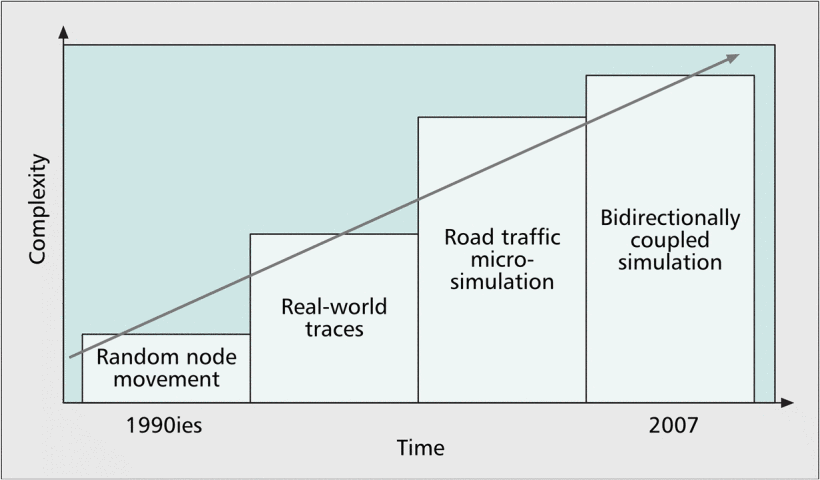
\includegraphics[width=\linewidth]{figuras/evolution_bidirectional_sim_sommerdressler.png}
    \caption{Evolución de simulaciones integradas para ITS (fuente: \autocite{sommer_dressler2}).}
    \label{fig:bidir_evol}
\end{figure}

La necesidad de un entorno integrado para la simulación de Sistemas Inteligentes de Transportes es un tema que ha estado presente en la comunidad académica hace casi más de una década ya. En particular, Sommer \emph{et al.} argumentaron fuertemente a favor de la idea en \autocite{bidirectionalsimul} y \autocite{sommer_dressler2}; el siguiente análisis se basa principalmente en ambos documentos, con algunas fuentes adicionales que se mencionarán oportunamente. 

En primer lugar, los autores destacan la existencia de un sistema de simulación bidireccional desarrollado por la Universidad Nacional de Chiao Tung, Taiwan \autocite{nctuns4,nctuns6}, el cual permite la simulación íntegra de un sistema de transportes dotado de capacidades de comunicación inalámbrica. 

\emph{NCTUns}, actualmente en su versión 6.0 (publicada en junio del 2010 \autocite{nctuns6}), es un simulador para el estudio de Sistemas Inteligentes de Transporte. Su principal particularidad es que presenta un entorno totalmente integrado para la ejecución de dichas simulaciones; es decir, es tanto un simulador de redes de comunicaciones como de tráfico. Incluye capacidades para simular comportamiento tanto autónomo como predefinido (\emph{rutas}) de vehículos, e implementa un \emph{stack} de protocolo completo en cada vehículo.

No obstante, Sommer \emph{et al.} critican la incompatibilidad de dicho sistema (en su versión 4.0) con los modelos de protocolos de comunicación y transporte ya desarrollados para los simuladores más prominentes, limitando su utilidad práctica en la investigación. Además. si bien NCTUns es capaz de simular un número capacidad de capas físicas, todavía se encuentra muy limitado en ese aspecto en comparación con otros simuladores de redes.

Los investigadores mencionan también la existencia de TraNS \autocite{piorkowski2008trans}, un \emph{framework} para la integración de ns-2 con SUMO. Este sistema implementa un \emph{loop} de control y \emph{feedback} activo entre ambos simuladores, estableciendo así una simulación bidireccional que permite la emulación de un ITS.

TraNS integra dos simuladores de renombre en la academia, y ha sido muy bien recibido. Sin embargo, los autores destacan que carece de ciertas funcionalidades -- principalmente, la capacidad de sincronizar y controlar el tiempo de simulación entre ambos simuladores.

Se debe destacar también los trabajos realizados por investigadores en la Universidad Estatal de Nueva York en Buffalo \autocite{zhao2016integrated} y de la Universidad de Düsseldorf \autocite{lochert2005multiple}. Ambos constituyen ejemplos de simulaciones bidireccionale -- no obstante se ven limitados por su especificidad, y dificultad de adaptación a escenarios más diversos. El trabajo de Shalaby en su tesis de magíster \autocite{shalaby} también sufre este mismo problema, además de temas relacionados a la eficiencia del \emph{framework} desarrollado por la autora, principalmente ligado a la elección de mecanismo de comunicación entre los simuladores (archivos en disco).


Finalmente, Sommer, German y Dressler presentan su solución en \autocite{sommer_german_dressler}: VEINS, un \textit{framework} de integración entre OMNeT++ y SUMO. Ambos simuladores se escogieron específicamente por su adopción en el mundo académico, y por sus naturalezas abiertas y fáciles de adaptar y modificar.

A través de VEINS, ambos simuladores se ejecutan en paralelo, comunicándose en tiempo real mediante un \textit{socket} utilizando el protocolo TCP; SUMO proporciona las trazas de movimiento de los elementos en la simulación a la vez que OMNeT++ simula el comportamiento de la red de comunicaciones. Además, mediante este esquema, OMNeT++ también puede modificar directamente el comportamiento del modelo de transporte, por ejemplo alterando la velocidad de un vehículo en respuesta a un mensaje específico obtenido a través de la red de comunicaciones. De esta manera, el \textit{framework} en cuestión permite modelar sistemas complejos y dinámicos, que reflejan de buena manera la realidad.

Sin embargo, VEINS sufre por su elección de simulador de transporte; SUMO todavía se encuentra en una temprana etapa de desarrollo, lo cual implica que frecuentemente sufre de problemas de estabilidad y de falta de características y documentación. Por ejemplo, hasta diciembre del 2015 (versión 0.25.0), SUMO no contaba con un editor gráfico de redes de transporte\footnote{\url{http://sumo.dlr.de/wiki/FAQ}}, lo cual dificultaba mucho el diseño de redes originales. Además, la curva de aprendizaje de SUMO es bastante pronunciada, y todas sus configuraciones son a través de archivos; es por esto que en muchos departamentos de ingeniería de transporte se opta por otros simuladores más avanzados y estables. 


